\chapter{Konzepterstellung}
\label{ch:konzept}
    Bei modernen Lüftungsanlagen ist davon auszugehen, dass Betriebsdaten an zentrale Einrichtungen, wie lokale Server zur Überwachung übermittelt werden. Es ist daher sinnvoll an dieser Stelle eine API einzurichten, welche Betriebsdaten an eine Servercloud oder lokale \ac{vm} zum Zweck der Analyse übermittelt. An dieser Datensenke kann dann ein Service zur KI-basierten Analyse bzw. Vorhersage von Schadensfällen eingesetzt werden. Eventuell lassen sich hierfür bereits genutzte Datenbanken einbinden, unter der Vorraussetzung, dass das \ac{ki}-Modell an das Datenmodell angepasst ist, oder alternativ eine Schnittstelle zur Modellierung eingesetzt wird. Die so gewonnenen Zeitverläufe lassen sich dann für die Prognose des Verschleißzustandes nutzen. Das Ziel des Konzeptes ist nicht eine Steuerung, oder Regelung, sondern eine Prognose auf Grundlage historischer und aktueller Zeitverläufe verknüpft mit Verschleißkennwerten. Sie ist somit unabhängig von Echtzeitdaten, und stellt folglich auch keine Echtzeitanforderungen an die Datenübertragung. Vielmehr fußt das Konzept auf Erfahrungswerten aus realen Tests oder robusten bzw. validierten mathematischen Modellen, wobei erstere immer zu einer genaueren Prognose führen werden. 
    Bei einer Anlage die mit Umluft oder Mischluft betrieben wird, werden zusätzliche Modelle erforderlich, die die in den Räumlichkeiten erzeugte Staubbelastung zusätzlich berücksichtigen, welche auf evtl. genormten Belastungen basiert.
    Moderne Anlagen werden als reine Außenluftanlage ausgelegt. Hierbei wird die Außenluft zentral aufbereitet und über ein Kanalnetz an die Räume geleitet. Die verbrauchte Luft wird über ein getrenntes Netz und Abluftventilator aus den Räumen transportiert, wobei im Sinne der Energieeffizienz in der Regel eine Wärmerückgewinnung für das Zuluftsystem erfolgt. \cite{tavg}
    Daher erfolgt die Entwicklung des Konzepts anhand eines reinem Außenluftbetriebes. Im Fort- und Abluftsystem einer solchen Anlage wird dann nur ein Filter zum Schutz des Abluftventilators eingesetzt, esseidenn, es greifen Emissionsschutzvorschriften durch in den Räumen auftrende Schadstoffe.
    Soll die erwartbare Auslastung, im Sinne einer State-of-the-Art Wartungsplanung (s. \ref{sec:predmain}), in die Vorhersage einfließen, werden auch für die Zuluft Informationen bezüglich Staubzusammensetzung und -Last erforderlich. 
\section{Beschreibung gewählter Filterbauart}
    Die in Kap. \ref{sec:auswahl_konk} gewählten Filter sind Tiefenfilter.
    Bei Tiefenfiltern treten allgemein folgende, bereits vorgestellte Filtereffekte auf \cite*{transportvorgänge}:
\begin{itemize}
    \item Sperreffekt
    \item Trägheitseffekt
    \item Diffusionseffekt
\end{itemize}
    Der Einfluss der Effekte schwankt hierbei je nach Volumenstrom, Filterklasse/-Art und Staubzusammensetzung. Entsprechende Kennlinien sind spezifisch für unterschiedliche Filter.Ein vollständiges Konzept müsste diese Einflüsse quantifizieren, um den Rahmen einer Studienarbeit nicht zu überschreiten wird der Volumenstrom im Sinne einer IDA-C4 Regelung gesteuert, die Staubzusammensetzung wird als konstant angenommen (s. \ref{sec:sim} ). 
    Da die Staubzusammensetzung und -konzentration ein bestimmender Faktor für die Beladung der Filter ist, und zeit- und ortsabhängig ist, müsste diese auch in das System einfließen. Dies ist mit Versuchen kaum reproduzierbar, weshalb eine Bewertung des Verschleißzustandes von insbesondere Außenfiltern im realen Betrieb anhand der realen Verläufe eben dieser Größen für die Umsetzung unabdingbar ist.
    Zum Zweck der Darstellung einer Machbarkeit wird nur der E11-Filter (Datenblätter s. Anhang) detaillierter untersucht. Für diesen liegt ausreichend Literatur vor, welche den Einfluss von z.B. Feuchte auf Druckdifferenzverläufe und Verschleiß untersucht. Die nötigen Genauigkeiten für die herausgearbeiteten Messgrößen werden hierbei schon von den meisten low-cost Sensoren erreicht. Eine Evaluation der Abtastraten entfällt, da hier eher minütliche Abtastungen erforderlich sind, was eventuell sogar den Einsatz batteriebetriebener Sensoren ermöglicht. Ausnahme bildet hier die Abtastung der Druckdifferenz im Kontext von möglichen Druckstößen durch Lastwechsel oder Windböen. Die Festlegung der Abtastraten erfordert hierbei Messdaten aus der Praxis, welche dem Verfasser nicht vorliegen.
    \section{Auswahl Sensorik}
    \label{sec:auswahl_sens}
    Ausgehend von Kapitel \ref{sec:ident_mess} müssen die Messgrößen der folgenden Unterkapitel erfasst werden. Im Sinne des Retrofitting bieten sich daher sog. Smarte Sensoren an, um die Möglichkeiten der \ac{lta} zur Messung von Parametern sinnvoll und kosteneffizient zu erweitern. \cite{hybride} Folgend werden jeweils Lösungen zur Messung der unterschiedlichen Parameter vorgestellt. Hierbei ist davon auszugehen, das bereits Einrichtungen zur Messung von Differenzdrücken bzw. Strömung vorhanden sind, aber nicht solche für Temperatur und Feuchte. Für die Größen Temperatur und Feuchte werden daher kompakte, batteriebetriebene Sensoren vorgeschlagen, welche im Verbund mit einem Gateway über Funk, und schließlich über das 4G Mobilfunknetz, Daten in eine Cloud übertragen können. Hierbei wird auch eine REST API bereitgestellt, welche den derzeit quasi-Standard für Event gesteuerte Softwaresysteme darstellt.
    \subsection{Feuchte und Temperatur}
    \label{sec:smartsens}
    Hervorzuheben ist bei diesem Sensor von Disruptive Technologies die extrem kleinen Abmessungen (s. Abb. \ref{fi:feuchtesensor}), sowie die Lebensdauer von etwa 15 Jahren. Durch die Unabhängigkeit von der Stromversorgung würden sich derartige Sensoren ohne großen Aufwand an neuralgischen Punkten der \ac{lta} integrieren lassen. Durch die angesprochene Cloud-Konnektivität würden sie überdies Daten an dem Ort bereitstellen, an dem das vorherig trainierte KI-Modell die Analyse der Daten und Vorhersage der Wartungsfälle übernimmt. Da Feuchte und Temperaturschwankungen naturgemäß eher langsame Vorgänge sind, ist hierbei eine Abtastrate im Minutenbereich ausreichend.
    \begin{figure}[H]
        \begin{center}
            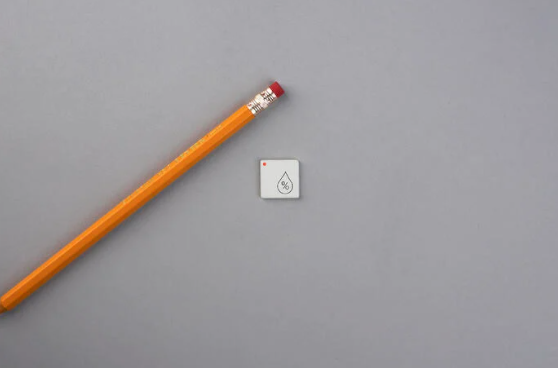
\includegraphics[width=0.8\linewidth]{images/feuchtesensor.png}
            \caption[Feuchtesensor]{Kabelloser Feuchte- und Temperatursensor von Disruptive Technologies \cite{disruptive} }
            \label{fi:feuchtesensor}
        \end{center}
    \end{figure} 
    \subsection{Volumenstrom}
    \label{sec:vstrom}
    Die Erfassung des Volumenstroms erfordert möglicherweise keine zusätzliche Messtechnik, wenn die entsprechenden Werte über die \ac{glt} lesbar sind, bzw. die zuständige Regelungstechnik ausreichend stabil und Netzwerk- oder Busfähig ist. Ist dies nicht gegeben bieten sich zwei verschiedene Lösungen an. Erstens eine Messung über Prandtl Staurohe, mit der Differenz zwischen statischem und dynamischen Druck. Hierbei muss die Messung temperaturkompensiert sein, was analog über eine Messbrücke oder digital über eine integrierte Temperaturmessung an selber Stelle möglich ist. Zweite Möglichkeit ist der Einsatz eines low-cost Strömungssensors, wie in Abbildung \ref{fi:strömsensor} vorgestellt. Durch den Analogausgang mit 0...10 V sollte dieser über Feldstationen in die \ac{glt} integrierbar sein. Ein Messbereich von 0...5\si{\metre\per\second}  sollte hierbei ebenfalls ausreichen. Die Genauigkeit vom vorgeschlagenen low-cost Sensor von $\mp 4\% $ ist hierbei annehmbar, da der Volumenstrom eher als Indikator für die Staubaufnahme zu sehen ist, und daher ohnehin mit einem Koeffizienten über die Zeit kumuliert werden muss.
    \begin{figure}[H]
        \begin{center}
            \includegraphics[width=0.5\linewidth]{images/strömsensor.png}
            \caption[Strömungssensor]{Richtungsunabhängiger low-cost Strömungssensor HLK100 von electro-mation \cite{strömsensor} }
            \label{fi:strömsensor}
        \end{center}
    \end{figure} 
    \subsection{Differenzdruck}
    Zur Messung von Differenzdrücken existieren am Markt eine Vielzahl von Sensoren. Diese Sensoren können ebenso zur Strömungsmessung (s. Kap. \ref{sec:vstrom}) eingesetzt werden.Beispielhaft wurde hier ein Modbus-fähiger Sensor (s. Abb \ref{fi:drucksensor}) ausgewählt. Dieser wäre im Sinne einer modernen \ac{glt} mit Bussystem sinnvoll. Um die Messdaten auch an eine Cloud übermitteln zu können, müsste folglich die zentrale Verarbeitungseinrichtung, wie Anfangs des Kapitels erwähnt, entsprechend ertüchtigt sein. Bei Druckdifferenz ist, im Gegensatz zu den anderen Messgrößen, evtl. eine höhere Abtastrate (Sekunden) nötig, um die in Kap \ref{sec:aufbau} erläuterten Druckschwankungen zu erfassen. Der Messbereich ergibt sich hierbei aus dem jew. Datenblatt, wobei ein Bereich von etwa 0...5 kPa sicherlich alle Fälle abdecken sollte. Dieser Bereich wird von dem vorgestellten Sensor abgedeckt. Die Genauigkeit des Sensors von $\mp 3\% EW$ reicht für den Zweck der Überwachung ebenfalls aus, da der Differenzdruck vermutlich als einer von vielen Grenzwerten realisiert wird. 
    \begin{figure}[H]
        \begin{center}
            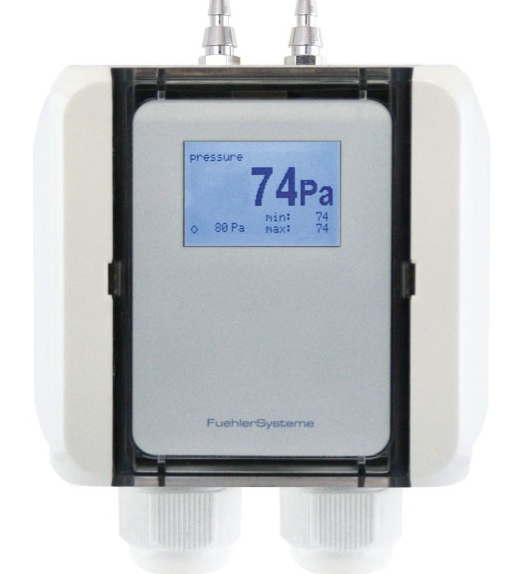
\includegraphics[width=0.5\linewidth]{images/drucksensor.png}
            \caption[Differenzdruck Messumformer]{Modbus-fähiger Drucksensor für Differenzdruck FS1200 von FühlerSysteme eNET \cite{drucksensor} }
            \label{fi:drucksensor}
        \end{center}
    \end{figure} 
    \section{Auswahl Systemarchitektur}
    Auf Basis (s. Kapitel \ref{sec:aufbau}) wird ein belegungsgesteuerter Volumenstrom mit zentraler Anlage angesetzt. Dies macht eine Erfassung von Volumenstromdaten erforderlich, um die Staubbeladung modellieren zu können. Die Frage an welchem Punkt im System dies geschieht, muss vom Aufbau der Anlage abhängig gemacht werden, es bietet sich jedoch an möglichst nah vor der Filtern derartige Messpunkte zu integrieren. Hierbei müssen eventuelle Leitungswiderstände aus der Oberfläche und Geometrie (Knicke etc.) der Schächte berücksichtigt werden. Bei Nutzung von KI ist dies jedoch nicht erforderlich, da diese Zusammenhänge von der KI "erlernt" werden können. Die Eingangsgrößen für das Modell wurden bereits in Kapitel \ref{sec:ident_mess} bzw. \ref{sec:umweltbed} erläutert. Die Messung von Klimadaten innerhalb der \ac{lta} sollte, unter der Annahme gleichbleibender bzw. vergleichbarer Werte innerhalb des Systems, kurz hinter dem Zuluftsystem ausreichen. Somit ist an den Filtern nur die Messung der Druckdifferenz einzusetzen, welche an Kanäle entsprechender Daten vom Zuluftsystem angebunden ist. Alternativ sind die Daten aus Zuluftsystem und Umgebung in einer lokalen Datenbank/Cloud verfügbar, und enstprechende \ac{api}'s z.B. zur Abfrage von Umweltdaten von Servern des Umweltbundesamtes eingerichtet (siehe \cite{webhookUBA}). Die Abbildung \ref{fi:architektur} zeigt hierbei die beispielhafte Umsetzung eines solchen Konzepts. Die relevanten Daten werden über unterschiedliche Protokolle an einen Cloud Server gesendet und dort analysiert. Es bietet sich in diesem Kontext an eine lokale Wetterstation in der Nähe der Zuluftseite außerhalb des Gebäudes zu installieren. Eine Wetterstation zu diesem Zweck ist in der Regel nicht kosteninstensiv, einfach zu installieren, und oftmals bereits für \ac{iot} Protokolle ausgerüstet und vorkonfiguriert. Die Messung von Differenzdrücken und Strömungsgeschwindigkeit wird über eine busfähige \ac{glt} an einen lokalen Server übermittelt, welcher die Daten über ein Webprotokoll an die Cloud weitergibt. Die Erfassung von Klimadaten innerhalb der Anlage erfolgt über die in Kapitel \ref{sec:smartsens} vorgestellten Smart Sensors. Da für die Abtastrate der Daten relativ geringe Anforderungen bestehen, ist die Wahl der Protkolle und \ac{api}'s hinsichtlich Bandbreite und Echtzeitfähigkeit unkritisch, und sollte anhand von Integrationsaufwand und Anschaffungskosten erfolgen.
    \begin{figure}[H]
        \begin{center}
            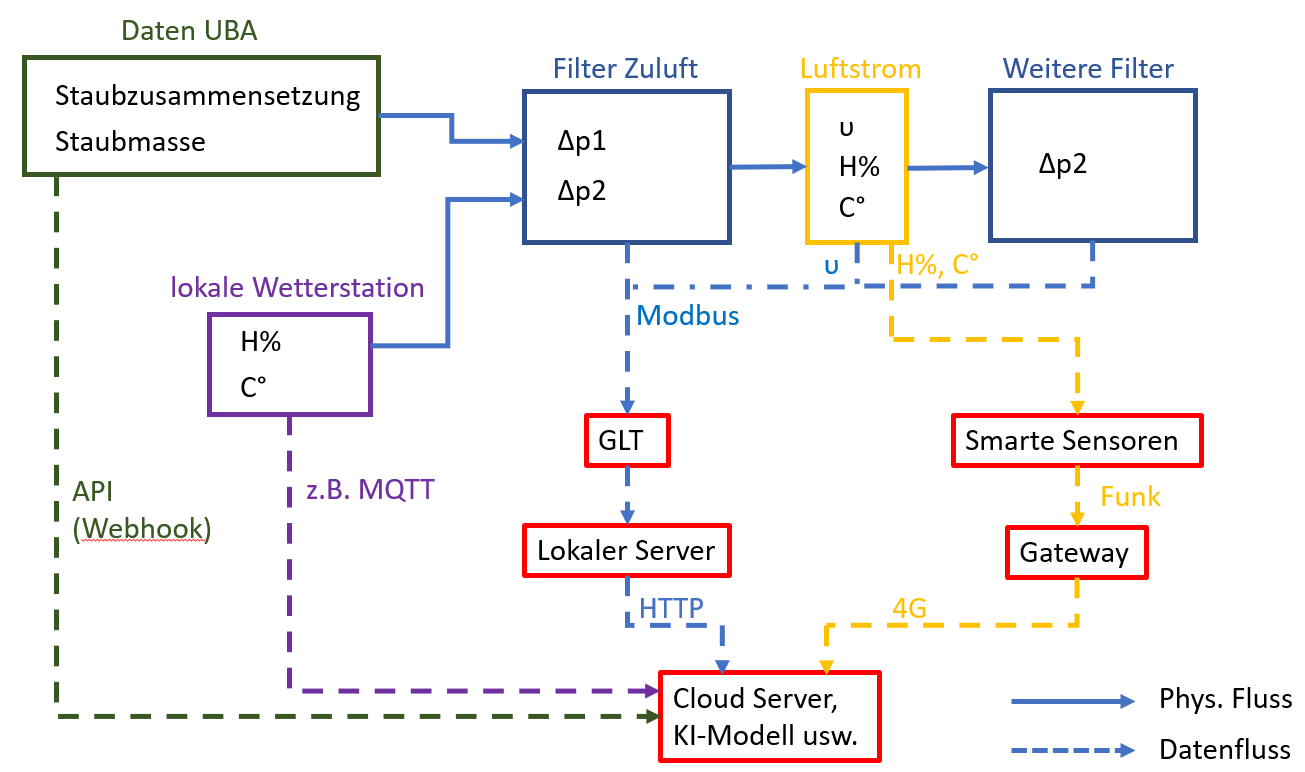
\includegraphics[width=\linewidth]{images/architektur.png}
            \caption[Architektur des Konzepts]{Beispielhafte Architektur des Konzepts}
            \label{fi:architektur}
        \end{center}
    \end{figure} 
    \section{Erforderliche Versuchsreihen}
    \label{sec:versuchsreihen}
    Angelehnt an die Untersuchungen von Bergmann \cite{hepa} und Ricketts \cite{feuchte} wäre es sinnvoll die bis zur Zerstörung erreichten Differenzdrücke an unterschiedlichen Proben der Filter zu untersuchen. Hierzu müssen konstante Prüfbedingungen, bestenfalls in Anlehnung an die Normen DIN EN ISO 16890 \cite{16890}, sowie DIN EN 1822 \cite{1822}, hergestellt werden.
    Optimal wäre es hierbei, Filterproben unterschiedlicher Einsatzdauer und hiermit verknüpfte, historische Daten zu den in Kap. \ref{sec:ident_mess} genannten Messgrößen, zerstörend zu prüfen, eventuell auch Zugversuche oder Berstdrucktests durchzuführen. Alternativ bzw. zusätzlich wären möglichst viele Versuchsreihen mit variablen Parametern sinnvoll, wenn dabei betriebsähnliche Bedingungen simuliert werden können. Hierbei wäre ein konstant halten der einzelnen Parameter nicht entscheidend für den Erfolg, sondern vielmehr die genaue messtechnische Erfassung und ausreichende Anzahl an Durchläufen, um eine zusätzliche Datenbasis für das KI-Modell zu generieren. Dies stellt auch den Vorteil einer KI-basierten Überwachung heraus, da hierfür nicht derselbe Aufwand betrieben werden muss, wie er nötig wäre um einzelne Zusammenhänge, z.B. den Einfluss von Luftfeuchte auf erreichte Enddruckdifferenzen, zu prüfen. Denn bei der Ermittlung derartiger mathematisch-physikalischen Zusammenhänge müssten bestimmte Einflussgrößen konstant gehalten werden, während andere variiert werden, was eine Entwicklung entsprechender Regelungen und Aktorik voraussetzt.
    \section{Funktionsweise}
    \label{sec:funktionsweise}
    Ziel des KI-Modells ist also die Vorhersage des Versagens eines Filters, bevor dieser auftritt, in einem bestimmten Vorhersagehorizont. Dieser Vorhersagehorizont ist abhängig von der Reaktionszeit bzw. den Gegebenheiten vor Ort, und kann auch von Kosten abhängig sein. Beispielsweise deckt ein Vorhersagehorizont von einer Woche mit Sicherheit Werktage ab, während bei einem kleineren Vorhersagehorizont evtl. zusätzliche Kosten durch z.B. Wochenendzuschläge entstehen können.
    Eingangsgrößen für die Vorhersage sind: Feuchte, Temperatur, Staubzusammensetzung, Volumenstrom und Druckdifferenz, wie in Kap. \ref{sec:auswahl_sens} und Kap. \ref{sec:ident_mess} vorgestellt. Die Standzeit kann durchaus ebenfalls relevant sein, wenn Alterungseffekte für das Filtermedium relevant sind. \\
    Allgemein wird der Vorhersagehorizont erreicht, in dem ein KI-Modell mit Fehlerdaten angelernt wird, die mit vergangenen Eingangsgrößen verknüft sind. In der Anwendung resultiert hieraus, dass die KI mit IST-Werten, innerhalb einer gewissen Unschärfe, die Zukunft vorhersagen kann. Hierbei müssen die Daten vorher aufbereitet werden, was z.B. Kumulation oder Mittelwertsbildung vergangener Werte eines Filters einschließt (s. Kap. \ref{sec:knime}). Die Festlegung dieser Aufbereitungsverfahren erfordert Domänenwissen, was durch die Analyse von bisherigen Verläufen und Kenntnisse über Luftfilter einschließt. Die Bereitstellung der Daten erfolgt auf Feldebene bestenfalls durch den Einsaz von Smart-Sensors (s. Kap. \ref{sec:auswahl_sens}), und die Verknüpfung darüber hinaus mit einer busfähigen \ac{glt}. Die Software \ac{KNIME} bietet hierfür bereits sowohl die Möglichkeit z.B. eine SQL-Datenbank abzufragen, in welcher die Messdaten gespeichert sein könnten, als auch die Möglichkeit Alarme über gängige Web-API's zu implementieren. Die konkrete Integration eines solchen Konzepts soll in dieser Arbeit nicht vorgestellt werden, da diese von zu vielen Umständen, wie vorhandene Serverinfrastruktur, Art der bisherigen Wartungsplanung(-software) usw., abhängig ist.